%!TEX root = Slic3r-Manual.tex

\section{Extrudeuse Multiple} % (fold)
\label{sec:multiple_extruders}
\index{extruders!multiple}
\index{extrudeuse!multiple}

Une imprimante avec plus d'une extrudeuse peut \^etre utilis\'e de diff\'erentes mani\`eres: L'extrudeuse suppl\'ementaire pourrait imprimer une couleur ou une mati\`ere diff\'erente, ou pourrait \^etre attribu\'e \`a l'impression de caract\'eristiques particuli\`eres, telles que le remplissage, le support ou les p\'erim\`etres.

L'impression multi-mati\`eres n\'ecessite un objet conçu de mani\`ere appropri\'ee g\'en\'eralement \'ecrits au format AMF qui peut g\'erer plusieurs mat\'eriaux (voir les mod\`ele de format au §\ref{sub:model_formats}).  Les d\'etails sur la façon de cr\'eer de tel fichier sont donn\'es ci-dessous.


\subsection{Configurer les Extrudeuses} % (fold)
\label{sub:configuring_extruders}
\index{Printer Settings!General!Capabilities!Extruders}
\index{Param\`etres de l'Imprimante!Fonctionnalit\'es!Extrudeuses}

Dans l'onglet \texttt{Printer Settings} (Param\`etres de l'Imprimante) il y a le param\`etre \texttt{Extruders} (Extrudeuses), dans la section \texttt{Capabilities} (Fonctionnalit\'es), ce qui permet de d\'efinir le nombre d'extrudeuses. Incr\'ementer cette valeur ajouter dynamiquement une autre d\'efinition d'extrudeuse dans le volet de gauche.

\begin{figure}[H]
\centering
\includegraphics[keepaspectratio=true,width=1\textwidth]{expertmode/multipleextruders/printer_settings_general_multiple_extruder_options.png}
\caption{Param\`etres d'Extrudeuses Multiples - Onglet Param\`etre de l'Imprimante (G\'en\'eral).  Notez les deux extrudeuses d\'efinies dans le volet de gauche.}
\label{fig:printer_settings_general_multiple_extruder_options}
\end{figure}

Chaque extrudeuse peut \^etre configur\'e comme d'habitude, mais il y a d'autres param\`etres qui doivent \^etre d\'efinis qui sont notamment les configurations multi-extrudeuse.

\begin{figure}[H]
\centering
\includegraphics[keepaspectratio=true,width=1\textwidth]{expertmode/multipleextruders/printer_settings_extruder_multiple_extruder_options.png}
\caption{Param\`etres d'Extrudeuses Multiples - Onglet Param\`etre de l'Imprimante (Extruder).}
\label{fig:printer_settings_extruder_multiple_extruder_options}
\end{figure}

\index{Printer Settings!Extruder!Extruder offset}
\index{Param\`etres de l'Imprimante!D\'ecalage de l'extrudeuse}

l'\texttt{Extruder offset} (D\'ecalage de l'extrudeuse) doit \^etre utilis\'e si le microprogramme ne g\`ere pas le d\'ecalage de chaque buse suppl\'ementaire. La documentation de votre micrologiciel devrait vous dire si c'est le cas. Chaque extrudeuse suppl\'ementaire a un d\'ecalage par rapport \`a la premi\`ere. Si le firmware le g\`ere, toutes les compensations peuvent rester \`a 0,0.

\index{Printer Settings!Extruder!Retraction!Length}
\index{Param\`etres de l'Imprimante!Extrudeuse!R\'etractation!Longueur}
Parce que l'extrudeuse secondaire sera en sommeil tandis que la premi\`ere est cours d'utilisation, et vice-versa, il est important que le mat\'eriau soit suffisamment r\'etract\'e pour cesser le suintement.  Comme avec les r\'eglages ordinaires de r\'etractation (voir p. \pageref{fig:retraction_settings}) le param\`etre \texttt{Length} (Longueur) est mesur\'e \`a partir du filament entrant dans l'extrudeuse.

% subsection configuring_extruders (end)

\subsection{Attribution de filaments} % (fold)
\label{sub:assigning_filaments}
\index{Plater}
\index{Surface de Travail}
Quand un profil d'imprimante avec plusieurs extrudeuses a \'et\'e s\'electionn\'e, l'onglet \texttt{Plater} (Surface de Travail) permet la s\'election d'un filament diff\'erent pour chaque extrudeuse.

\begin{figure}[H]
\centering
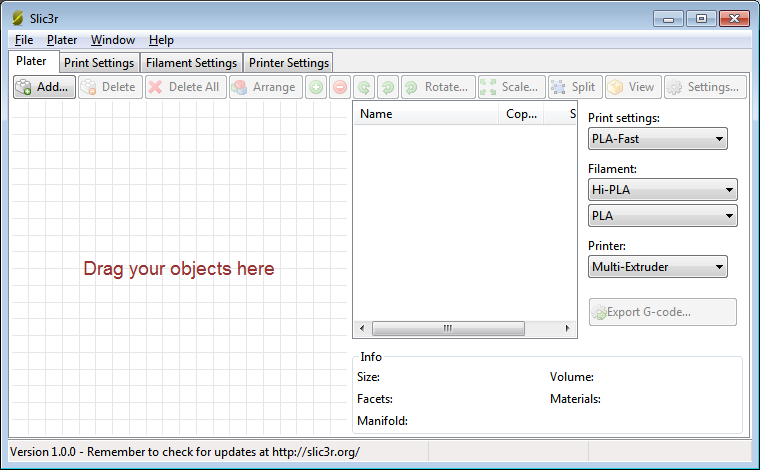
\includegraphics[keepaspectratio=true,width=1\textwidth]{expertmode/multipleextruders/plater_multi_filament.png}
\caption{Surface de travail avec de multiple param\`etre de filaments.}
\label{fig:plater_multi_filament}
\end{figure}

% subsection assigning_filaments (end)

\subsection{Affectation des extrudeuses pour les objets mono-mati\`ere} % (fold)
\label{sub:assigning_extruders}
\index{Print Settings!Multiple Extruders}
\index{Param\`etres de l'Imprimante!Extrudeuse Multiple}

Pour les impressions de mat\'eriaux unique, o\`u l'extrudeuse secondaire a pour mission une extrusion particuliere, la section \texttt{Multiple Extruders} (Extrudeuses multiples) de l'onglet \texttt{Print Settings} (Param\`etres de l'imprimante) donne la possibilit\'e d'assigner une extrudeuse pour chaque type d'extrusion.

\begin{figure}[H]
\centering
\includegraphics[keepaspectratio=true,width=1\textwidth]{expertmode/multipleextruders/print_settings_multiple_extruder_options.png}
\caption{Param\`etres d'Extrudeuse Multiple - Onglet Param\`etre d'Impression.}
\label{fig:advanced_multiple_extruder_options}
\end{figure}

% subsection assigning_extruders (end)

\subsection{Configurer le Changement d'Outil} % (fold)
\label{sub:configuring_tool_changes}

\index{Printer Settings!Custom G-code!Tool change G-code}
\index{Param\`etres de l'Imprimante!G-code personnalis\'e!G-code de changement d'outil}

La section \texttt{Custom G-code} (G-code personnalis\'e) de l'onglet \texttt{Printer Settings} (Param\`etres de l'Imprimante) dispose d'une option d'insertion de G-code entre les changements d'outils. Comme avec toutes les sections personnalis\'e G-code, les variables d'environement peuvent \^etre utilis\'ees afin de r\'ef\'erencer les param\`etres Slic3r.  Cela inclus les variables [previous\_extruder] et [next\_extruder].

\begin{figure}[H]
\centering
\includegraphics[keepaspectratio=true,width=1\textwidth]{expertmode/multipleextruders/printer_settings_custom_gcode.png}
\caption{Param\`etres d'Extrudeuse Multiple - G-code de Changement d'outil.}
\label{fig:printer_settings_custom_gcode}
\end{figure}

% subsection configuring_tool_changes (end)


\subsection{Impression d'objets multi-mati\`eres} % (fold)
\label{sub:printing_multi_material_objects}

Si un fichier multi-mat\'eriaux AMF existe d\'ej\`a, parce que le programme de CAO peut exporter un tel format, alors celui-ci peut \^etre charg\'e dans Slic3r de façon habituelle. Le mappage entre mati\`eres de l'objet et les extrudeuses est s\'equentielle, c'est \`a dire que la premiere mati\`ere est affect\'e \`a la premi\`ere extrudeuse, etc.

% subsection printing_multi_material_objects (end)


\subsection{G\'en\'eration de fichiers AMF multi-mati\`ere} % (fold)
\label{sub:generating_multi_material_amf_files}

Slic3r a la capacit\'e de combiner plusieurs fichiers STL dans un fichier multi-mati\`ere AMF.

\index{Menu!Combine multi-material STL files...}
\index{Menu!Combiner des fichiers STL multi-mati\`ere...}

\begin{itemize}
    \item Diviser la conception originale dans les diff\'erentes parties au sein du programme de CAO, et exporter chaque partie en STL.
    \item Dans Slic3r, choisissez \texttt{Combine multi-material STL files...} (Combiner des fichiers STL multi-mati\`ere...) \`a partir du menu \texttt{File} (Fichier).
    \item Lorsque vous \^etes invit\'e avec une bo\^ite de dialogueChoisissez le premier STL, qui sera attribu\'e \`a la premi\`ere mati\`ere (et donc la premi\`ere extrudeuse). Cliquez sur \texttt{Open} pour \^etre invit\'e au prochain STL, et ainsi de suite jusqu'\`a ce que chaque STL soit affect\'es \`a une mati\`ere. Pour signaler qu'il n'y a plus de fichiers STL, choisissez \texttt{Cancel} (Annuler).
    \item La bo\^ite de dialogue suivante demande l'emplacement et le nom du fichier de l'AMF.
\end{itemize}

Une fois g\'en\'er\'e le fichier peut \^etre charg\'e et imprim\'e comme d\'ecrit ci-dessus.

% subsection generating_multi_material_amf_files (end)

% section multipe_extruders (end)
